\chapter{Design}

    \paragraph*{}
        A significant amount of time was spent on the design of the system.
        A careful consideration was given to working of the frontend and the backend. The system was designed to be as modular as possible.
        The system was designed to be able to be used in multiple ways.
        Special attention to the design of the frontend was given including contrast ratios, colors and rhythm was given. User experience was also given a high priority. 



    \section{Design Patterns}
        \begin{itemize}
            \item{State}

            The useState hook in react exposes a way to change the state of the component, this allows us to re-render the ui whenever change the state of the component. The functional component might behave differently depending on the state of the component. This is how a the state pattern is used here.
            
            \begin{figure}[h]
                \centering
                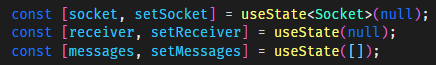
\includegraphics[width=0.8\textwidth]{images/useState.png}
                \caption{State Pattern}
                \label{fig:state}
            \end{figure}

            \pagebreak

            \item{Memento}
            
            The useMemo hook allows us to memoize the output of the component. This is how the memento pattern is used here. Here we are memoizing the slotList. This is done to avoid re-calculating and re-sorting the slotList when the component re-renders.

            \begin{figure}[h]
                \centering
                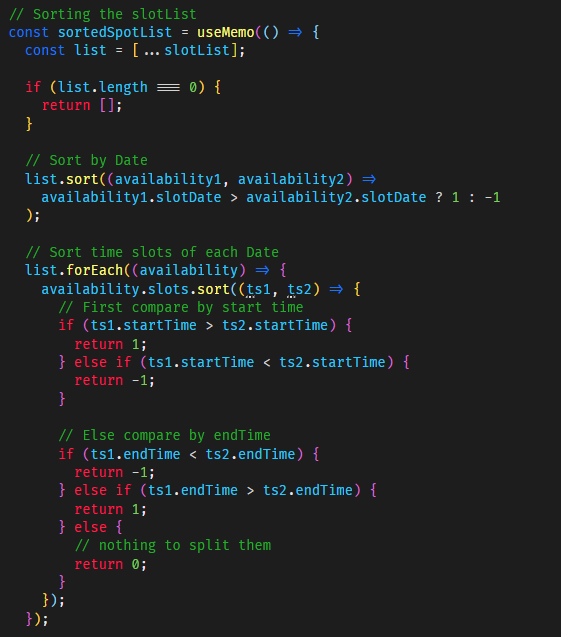
\includegraphics[width=0.8\textwidth]{images/useMemo.png}
                \caption{Memento Pattern}
                \label{fig:memento}
            \end{figure}
            
        \end{itemize}

        \pagebreak

        \section{Frontend}
           \subsection{Wireframe}
                \paragraph*{}
                    Before the development of the UI the design of the wireframe was considered. A wireframe of the UI was created that gave the general understanding of how the UI will be broken into components.

                    \begin{figure}[h]
                        \centering
                        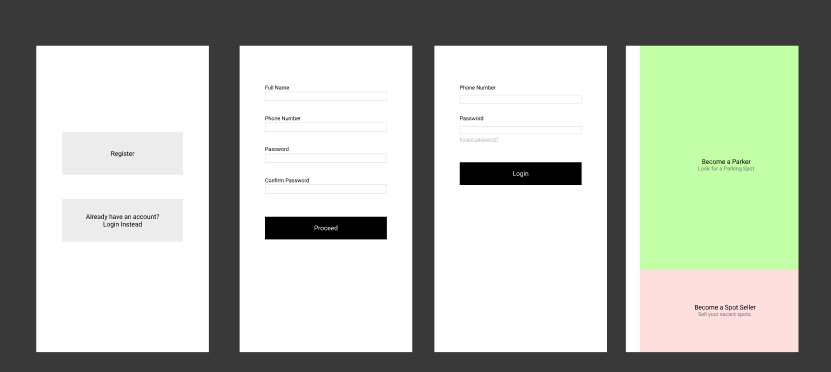
\includegraphics[width=0.6\textwidth]{images/homepageWireframe.png}
                        \caption{Homepage Wireframe}
                        \label{fig:homepageWireframe}
                    \end{figure}
 
                    \begin{figure}[h]
                        \centering
                        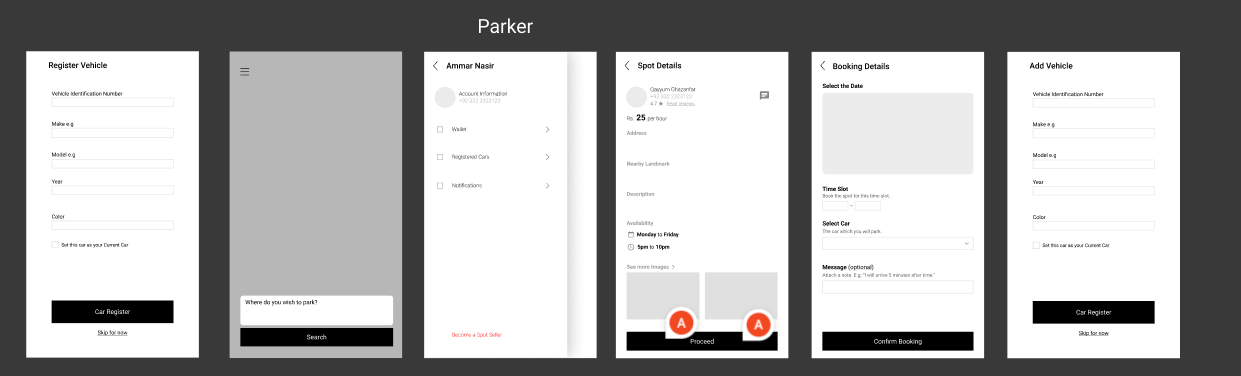
\includegraphics[width=0.6\textwidth]{images/parkerWireframe.png}
                        \caption{Parker Wireframe}
                        \label{fig:parkerWireframe}
                    \end{figure}

                    \begin{figure}[h]
                        \centering
                        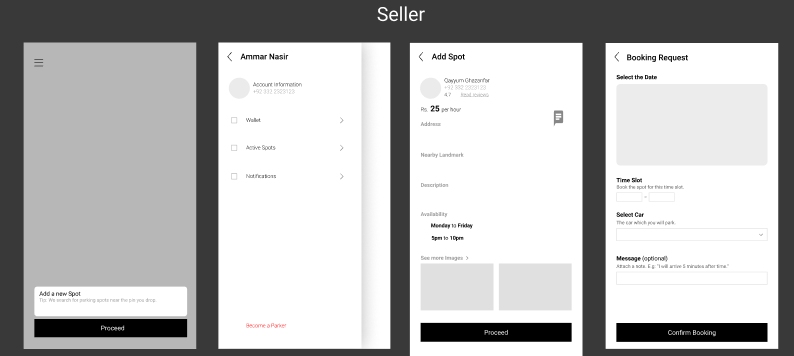
\includegraphics[width=0.6\textwidth]{images/sellerWireframe.png}
                        \caption{Seller Wireframe}
                        \label{fig:sellerWireframe}
                    \end{figure}

            \pagebreak
                \subsection{UI}
                \paragraph*{}
                    At the start of UI design the Font, Colors and Design schemes were solidified to ease the process and keep the consistency throughout the application. The aim was to make the UI look and feel like one cohesive application.

                    \begin{figure}[h]
                        \centering
                        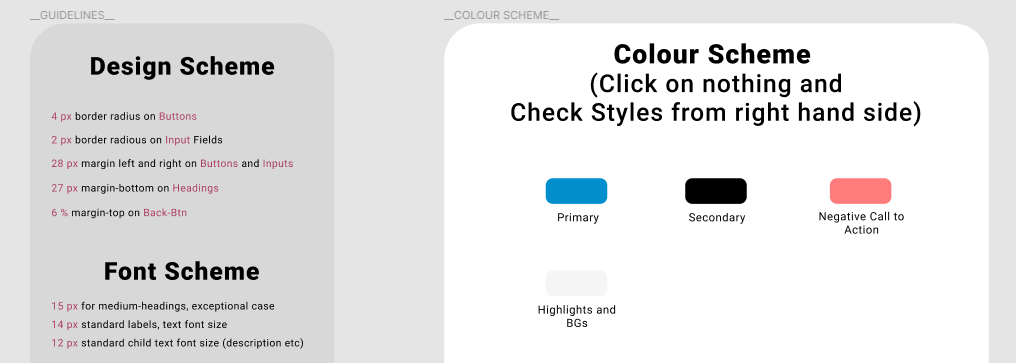
\includegraphics[width=0.8\textwidth]{images/colorScheme.png}
                        \caption{Color, Font, Design Schemes}
                        \label{fig:colorScheme}
                    \end{figure}
    
                    \begin{figure}[h]
                        \centering
                        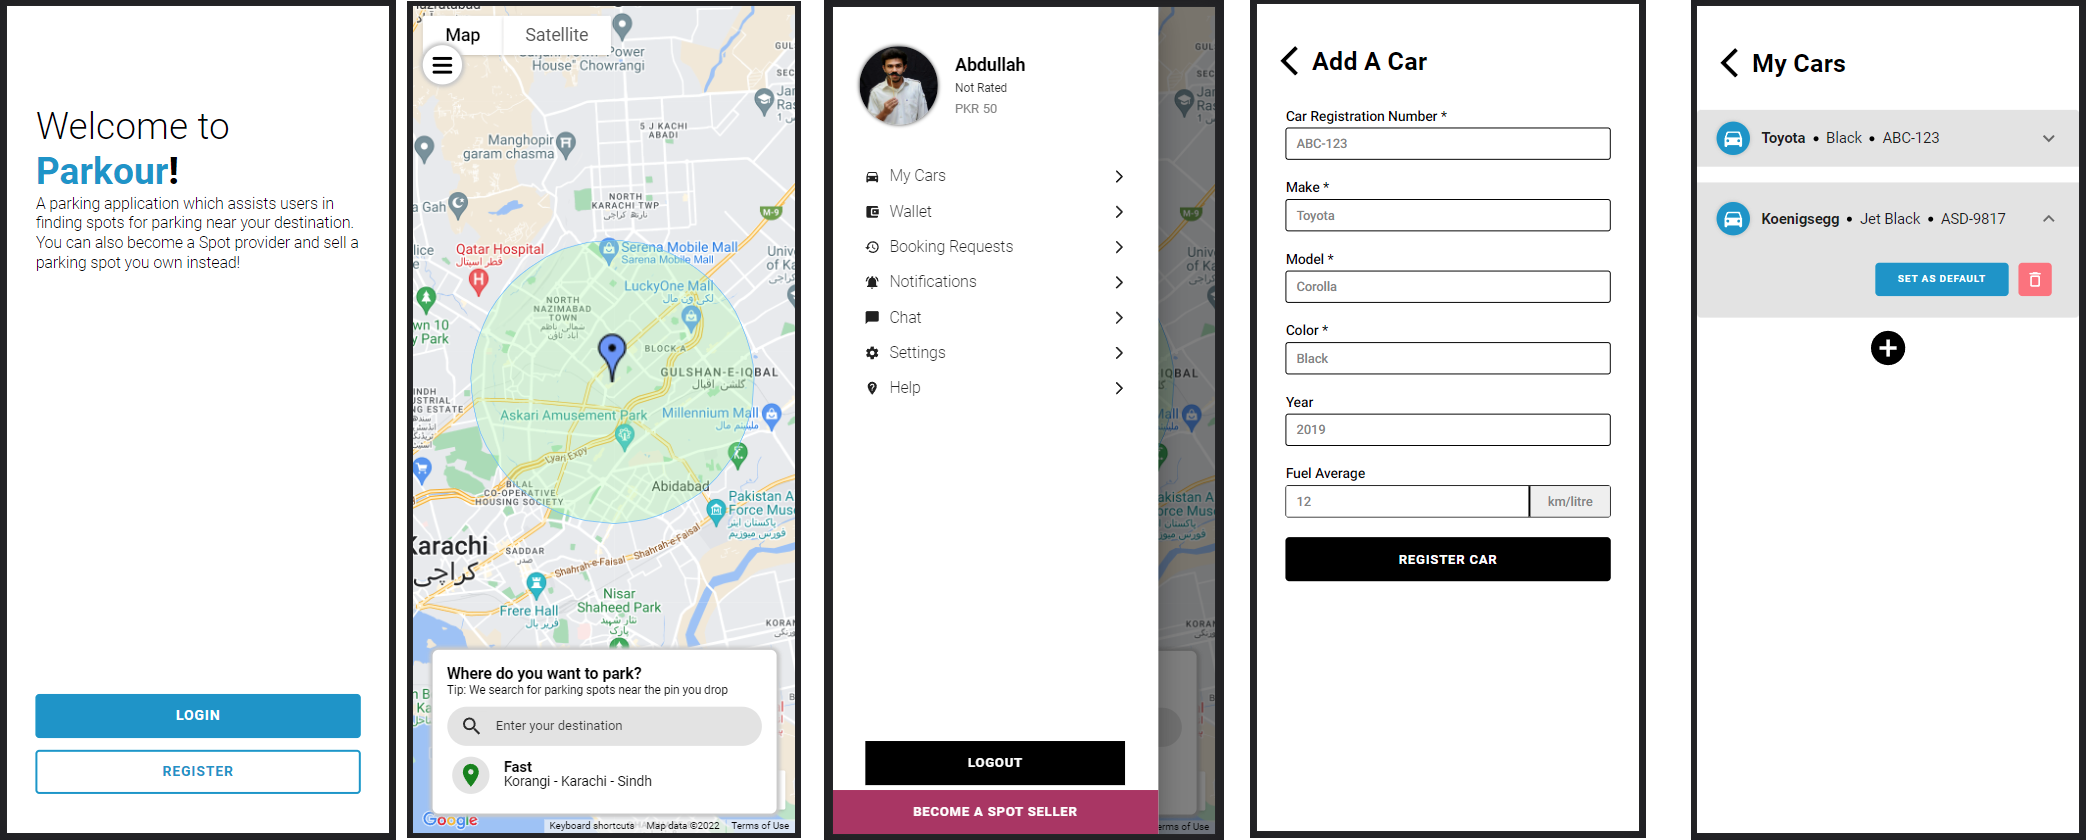
\includegraphics[width=0.8\textwidth]{images/ui1.png}
                        \caption{UI (1)}
                        \label{fig:ui1}
                    \end{figure}

                    \begin{figure}[h]
                        \centering
                        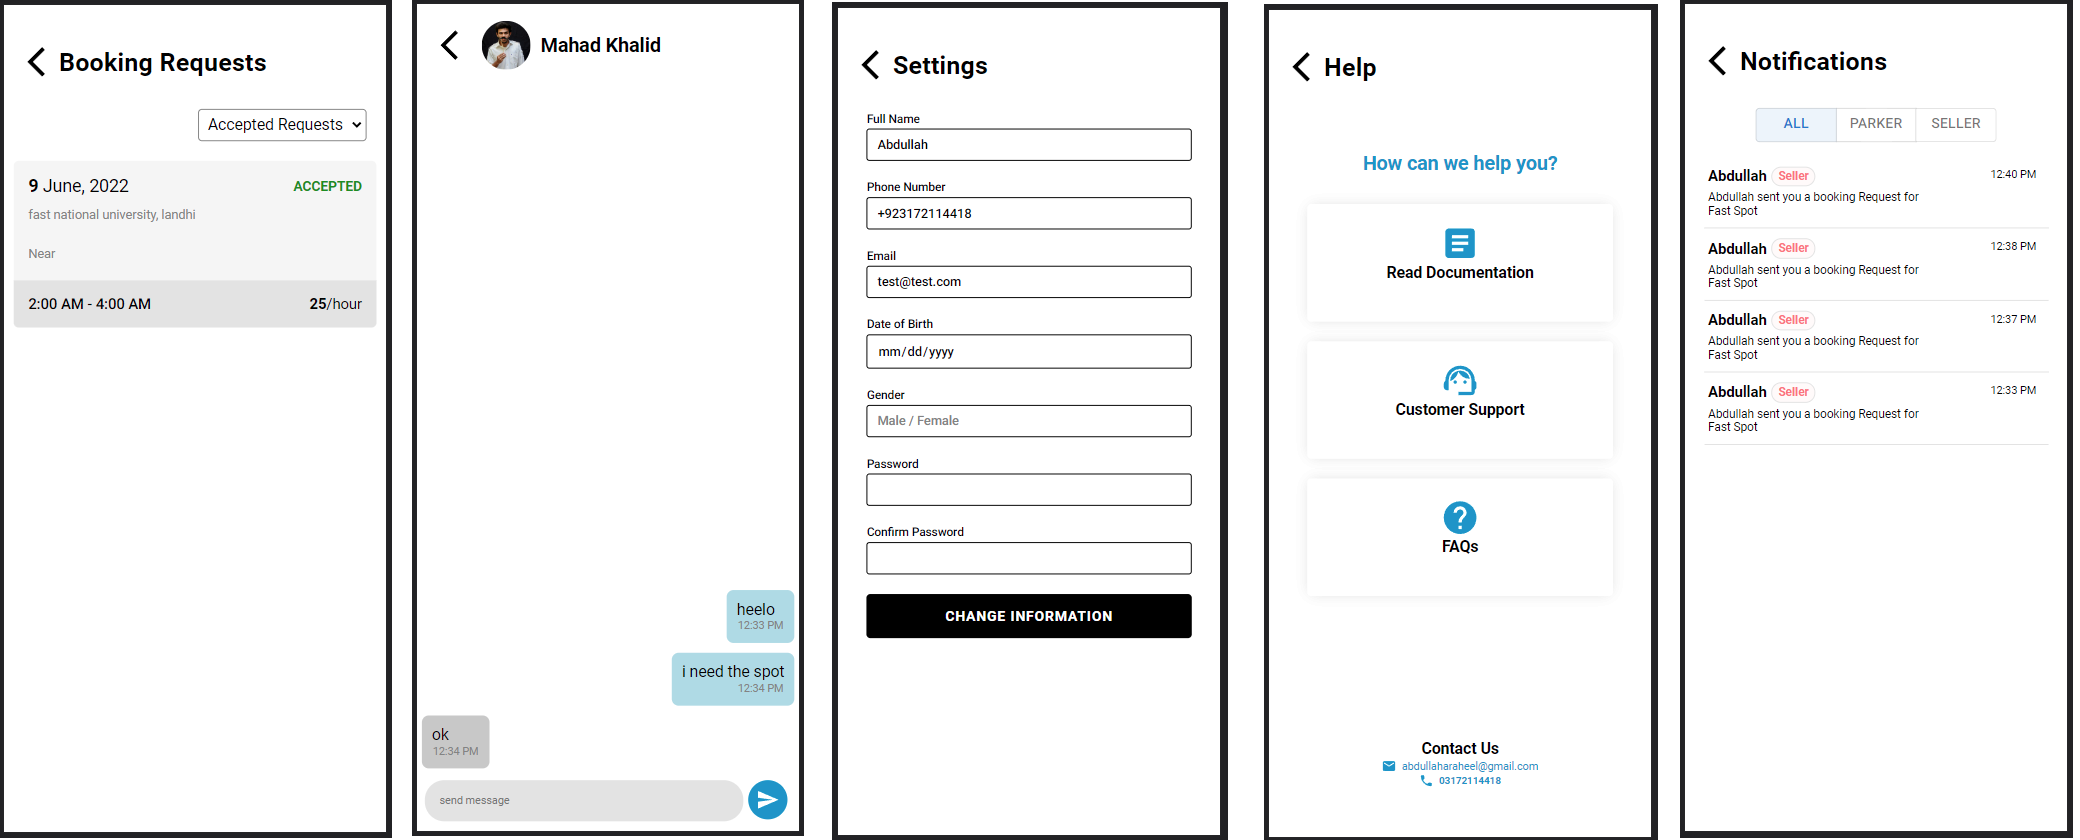
\includegraphics[width=0.8\textwidth]{images/ui2.png}
                        \caption{UI (2)}
                        \label{fig:ui2}
                    \end{figure}

                    
                    \begin{figure}[h]
                        \centering
                        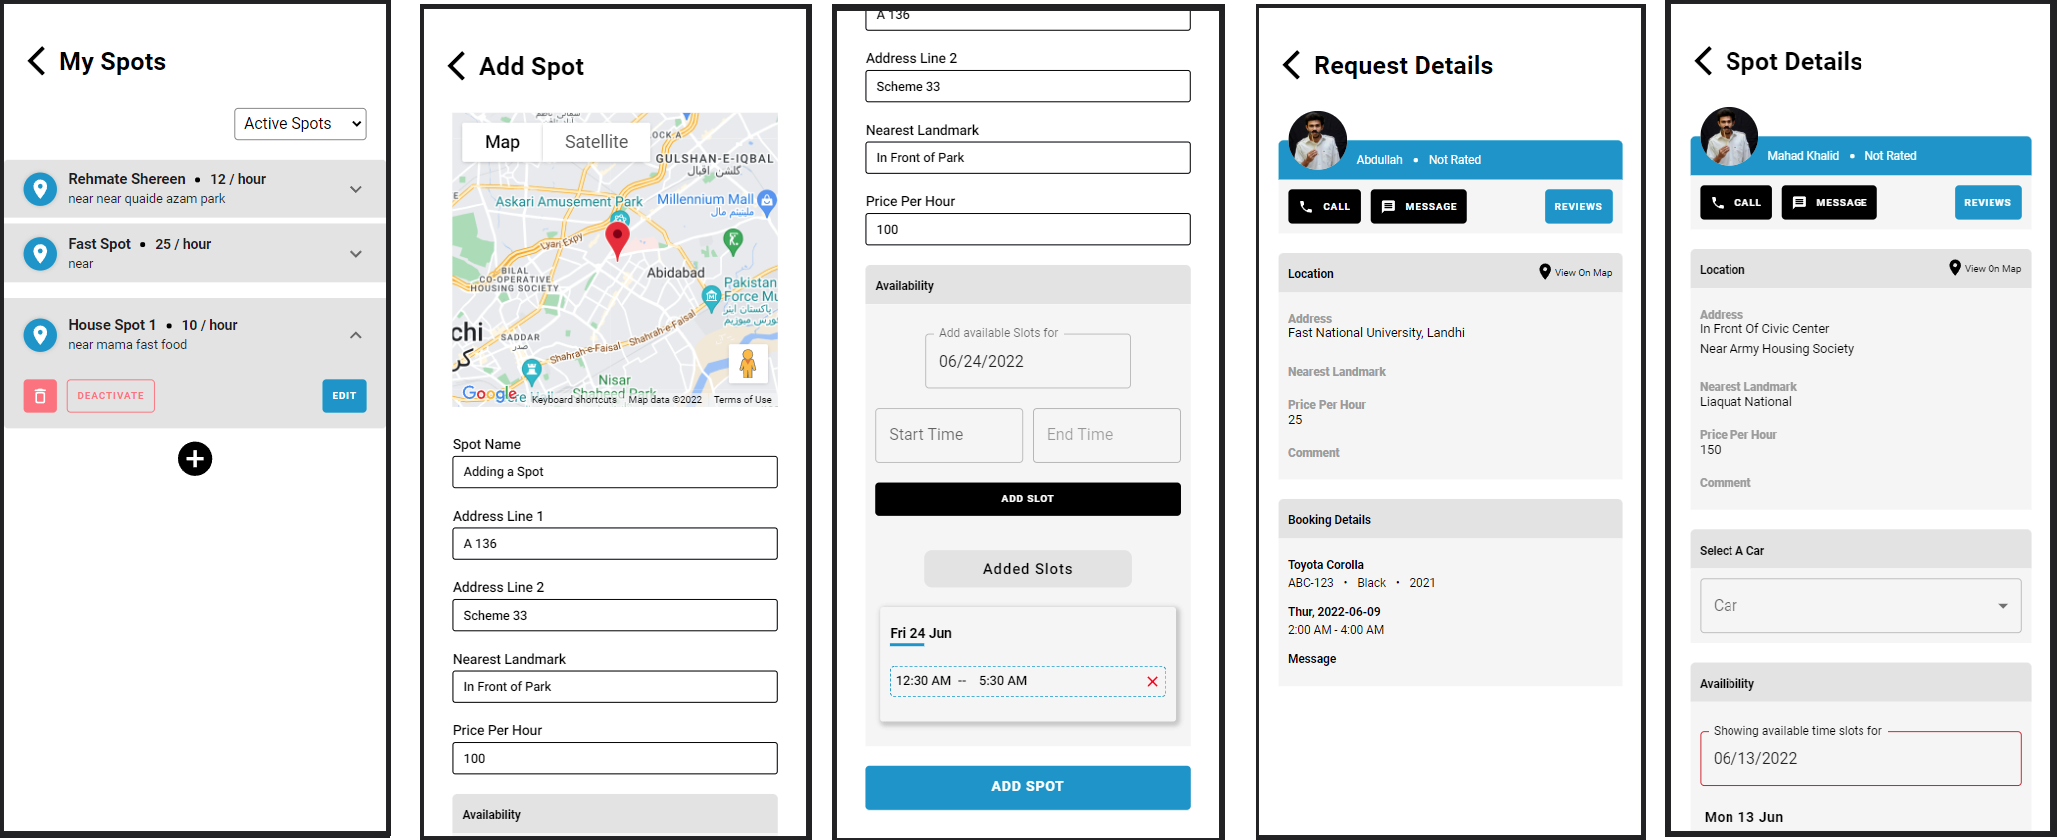
\includegraphics[width=0.8\textwidth]{images/ui3.png}
                        \caption{UI (3)}
                        \label{fig:ui3}
                    \end{figure}

                \pagebreak
                \clearpage
                    
                \section{Backend}
                    The design was planned considering the User Experience. Every effort is made to create a flexible data management method. An Example includes, maintaining history of data entities, time stamps, quality of life data.
                   \begin{figure}[h]
                        \centering
                        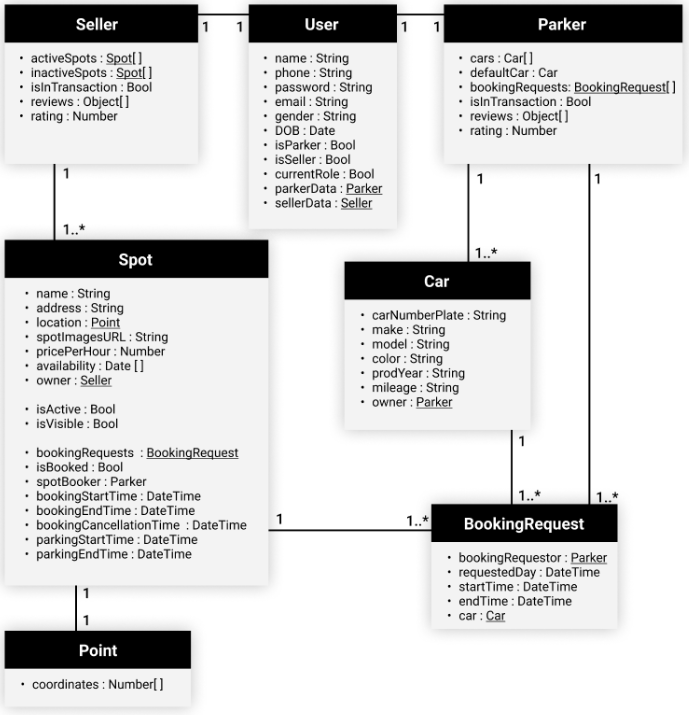
\includegraphics[width=0.8\textwidth]{images/dbDesign.png}
                        \caption{Database Design}
                        \label{fig:dbDesign}
                   \end{figure}

                    \pagebreak
                    \clearpage
                    
                    
                    Described the models in the following table.
                    \begin{table}[htb]
                        \centering
                        \begin{tabular}{ | l | p{125mm} |}
                            \hline
                            Model & Description \\
                            \hline
                            \hline
                            User & Schema containing personal information. Through sub documenting, the information of the user's "seller" and "parker" accounts is also stored here.\\
                            \hline
                            Parker & All user attachments related to their "parker" role, along with transactional parker states. \\
                            \hline
                            Seller & All user attachments related to their "parker" role, along with transactional parker states. \\
                            \hline
                            Car & Parker's car data to be shown in transactions. \\
                            \hline
                            Spot & Seller's spot data, its location, images, status, ratings etc. \\
                            \hline
                            Booking Request & Purely transactional data relating to parker's request and the spot requested. \\
                            \hline
                            Notification & Used to cache notifications  \\
                            \hline
                            Chat & The model that contains all the information about chat between parkers and sellers. \\
                            \hline
                        \end{tabular}
                        \caption{Models}
                        \label{tab:models}
                    \end{table}



                
        \pagebreak
        \section{Architecture}
        \paragraph*{}
        System handles Parker and Seller Interfaces separately. Sellers and Parkers will be able to indulge in transactions which are described as ‘a Parker finding a parking spot and finding one, and a seller listing their vacant parking spot for sale.’\\
        \paragraph*{}
        Both Parker and Seller will have digital in-app wallets to track their earnings/credits. Sellers will be able to cash in their credit after a certain number of conditions have been met.

        \subsection{Interface}
        \paragraph*{}
        The Interface was designed to be as user friendly as possible.
        The interface was designed to deliver the best user experience possible.\\

        \begin{figure}[h]
            \centering
            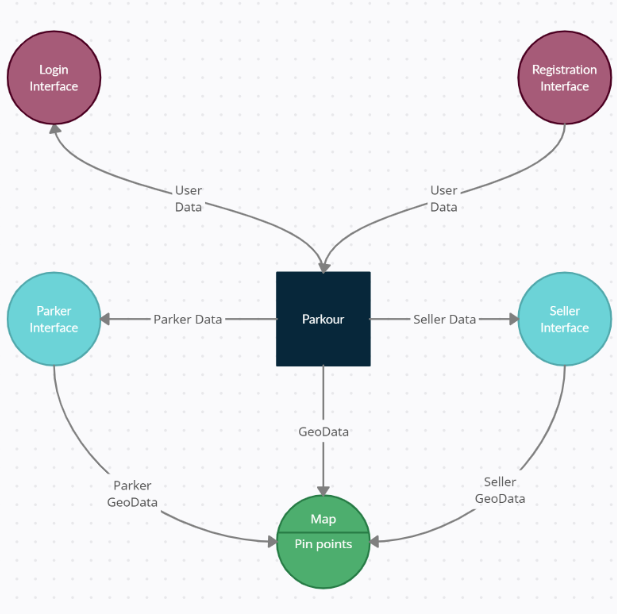
\includegraphics[width=0.7\textwidth]{images/externalInterface.png}
            \caption{Interface}
            \label{fig:interface}
        \end{figure}


        \pagebreak

        \subsection{Server}
        \paragraph*{}
            The server processes all the request form the frontend and makes changes to database accordingly.
            The server also authenticates user and makes sure that the user is logged in.\\
            The server also handles the booking request and the notification.\\
            The server also handles the chat.\\
            The server sends a response on each request.

            \begin{figure}[h]
                \centering
                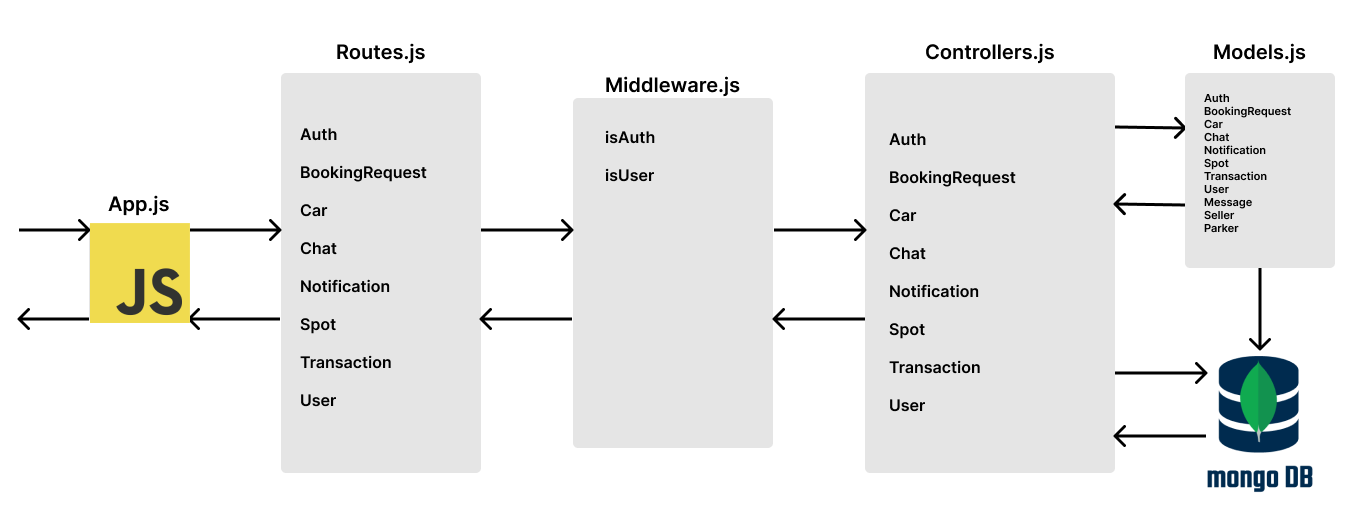
\includegraphics[width=0.8\textwidth]{images/server.png}
                \caption{Server}
                \label{fig:server}
            \end{figure}


            \pagebreak

            \subsection{Client}
            \paragraph*{}
                The client makes API calls to the server as well as the Goolge Maps server. The client makes use of redux to store information that can be used throughout the application.\\
    
                \begin{figure}[h]
                    \centering
                    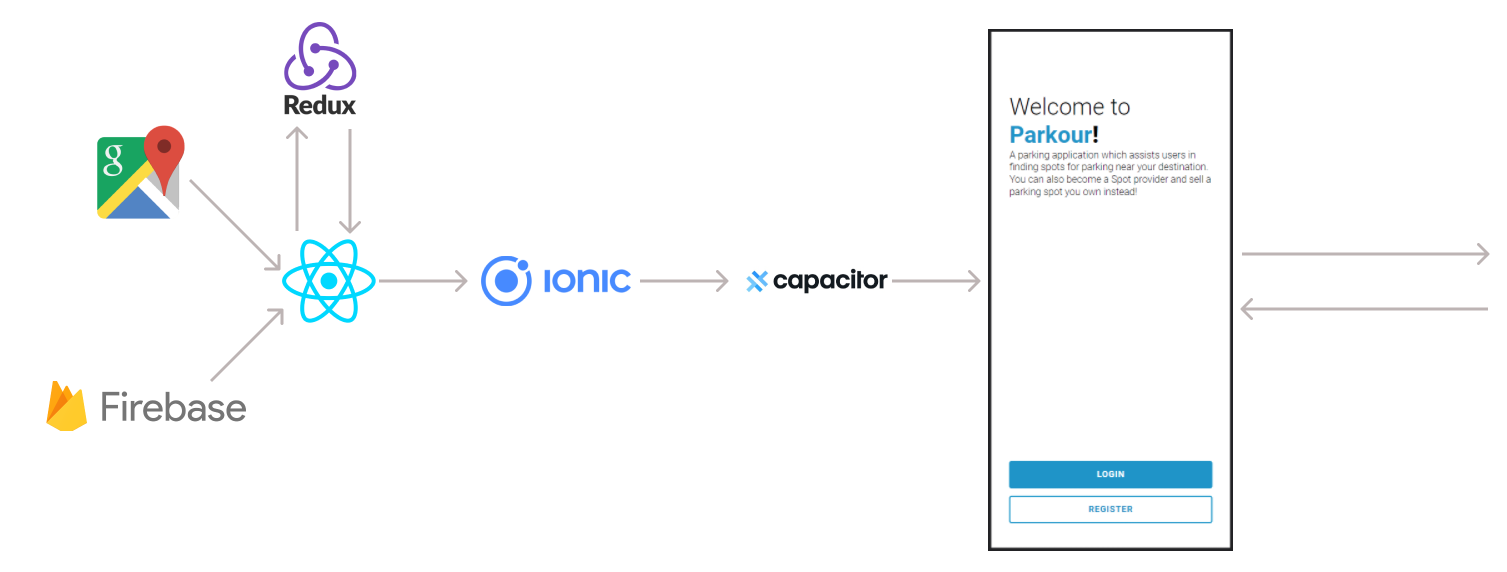
\includegraphics[width=0.8\textwidth]{images/FE_Architecture.png}
                    \caption{Client}
                    \label{fig:FE_Architecture}
                \end{figure}



                \subsection{Application}
                \paragraph*{}
                 The interaction between client and the server. \\
        
                    \begin{figure}[h]
                        \centering
                        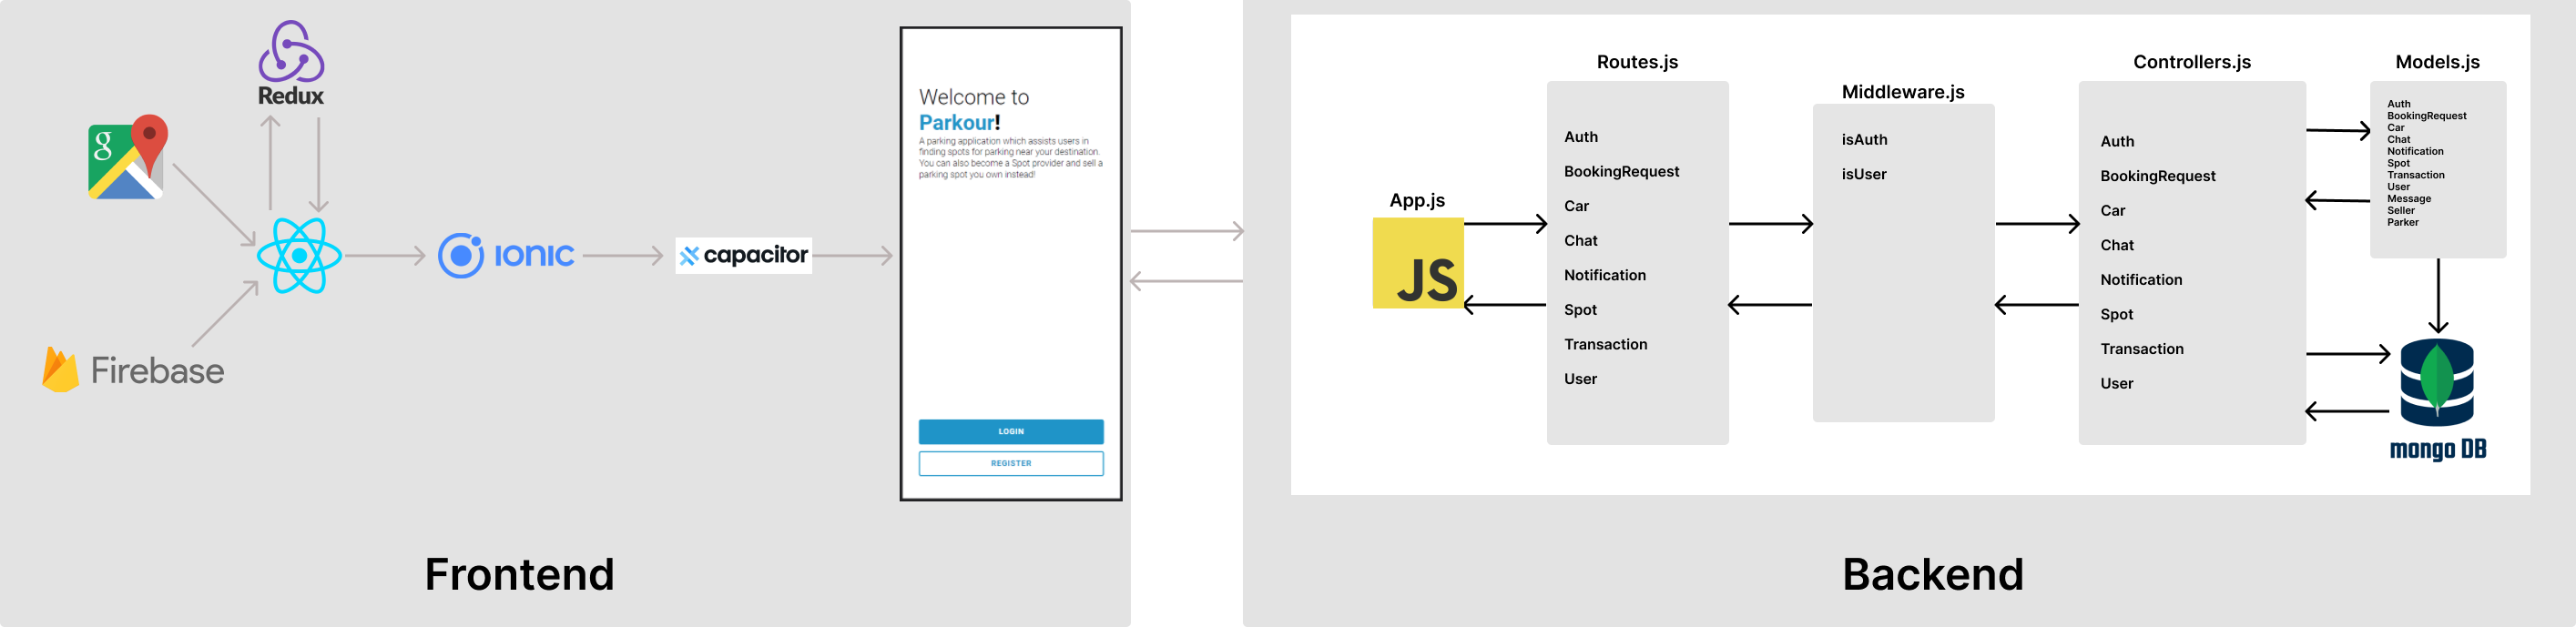
\includegraphics[width=1\textwidth]{images/WholeArcitectrue.png}
                        \caption{Application Architecture}
                        \label{fig:Architecture}
                    \end{figure}

